\textbf{Change this introduction to fit the final product!}
In this one year long project, we have collected results of a great number of materials with various structures and compositions. The initial experimentation was based on high-entropy silicides of the $Fe_2Si$ unit cell, created from the special quasi-random structure approach as described above. Despite the non-semiconducting character of this compound, we worked under the idea that the extraordinary properties that have been observed in high-entropy alloys through effects such as the cocktail effect, we could discover specific combinations of elements that would yield a semiconductor. In addition, the ratio between silicon atoms to metals allowed us to create nearly eqvimolar high-entropy alloys. 

Following this attempt, we transitioned into studying high-entropy silicides based on well known semiconducting 3d silicides such as $\beta-$\ch{FeSi2}, \ch{CrSi2} and \ch{MnSi_{1.75}}. The main outcome of this project is that for all 4 different starting silicides, we could only produce high-entropy silicides from one unit cell, furthermore in this cell only one specific compositions of elements was semiconducting. This was \ch{Cr_{0.25}Fe{0.25}Mn_{0.25}Ni_{0.25})Si2}, here-in CFMN, in the $\beta-$ \ch{FeSi2} crystal structure.  

This section will be structured in the following manner, firstly we will investigate the CFMN (fesi2) compound and various permutations of the composition. Thereafter we will look at other possible compositions of fesi2 based high-entropy silicides, and lastly test the CFMN composition in other crystal symmetries. In final we will present an overview of the complete study and the various compounds that have been investigated in order to propose promising directions and guideline future research directions in this field. In this way, we aim to understand the uniqe properties of CFMN (fesi2) and why this particular compound is semiconducting compared to the other testes structures in this project. Properties we will cover is the overall stability by total energy and corresponding enthalpy of formation, the magnetic properties and which elements contribute to the magnetism. But in majority, we will look at the band gap and related properties, as this is the main motivation and distinction of the study.    

\chapter{The results of \ch{(CrFeMnNi)Si2} in the $\beta-$\ch{FeSi2} structure}
\label{sec:good}

$\beta-FeSi_2$ in the orthorombic cmce crystal lattice is a well known semiconductor with an experimentally measured band gap of around 0.85 ev at room temperature \cite{PhysRevB.58.10389}, the nature of the band gap is under debate, all though most ab inito studies point to an indirect gap, experimental work indicate a direct gap. From our calculations we find an indirect band gap close to 0.65 eV with PBE, compared for example materials project's listed value of 0.698 eV with the same functional. Moreover in agreement with the calculations of materials project we discover that bulk $\beta-$ \ch{FeSi2} is diamagnetic. Finally, the enthalpy of formation of this compound is calculated as $-18.6583 eV$.

The high-entropy alloys generated from the \ch{FeSi2} unit cell alloys can be seen in figure 6.1. The supercells consist of 48 atoms each, in which the 16 iron sites is occupied equimolarly between Cr, Fe, Mn, and Ni, and the 32 silicon sites is as before occupied by silicon. Bellow in table 7.1 we list the enthalpy of formation ($\Delta H^0$) in addition to the total energy per atom (Toten), final magnetic moment per atom (Mag), and the band gap, for the five distinct SQSs plus the mean and standard deviation of the set. For simplicity, we denote the 5 supercells as A, B, C, D and E respectively.

\begin{table}[H]
\centering
\begin{tabular}{@{}cccc@{}}
\toprule
Structure  & Toten (eV) & Mag ($\mu_B$) & Band gap (eV) \\ \midrule
\textbf{A} & −6,6080                & 0.0833                    & 0.0280        \\
\textbf{B} & −6,6138                & 0.0833                    & 0.0523        \\
\textbf{C} & −6,6063                & 0.0834                    & 0.0344        \\
\textbf{D} & −6,6155                & 0.0833                    & 0             \\
\textbf{E} & −6,6089                & 0.0833                    & 0.0495        \\ \midrule
\textbf{Mean} & -6.6105 & 0.0833 & 0.0328    \\
\textbf{Std} & 0.0039 &  0.0000 &  0.0210 \\
\textbf{$\Delta H_{mean}^0$} & -11.5000 eV & - & - \\ \bottomrule
\end{tabular}
\caption{Total energy per atom, final magnetic moment, band gap (GGA) and formation enthalpy of $Cr_4Fe_4Mn_4Ni_4Si_{32}$ SQSs based on $FeSi_2$}
\label{table:fesi2_summary}
\end{table}  

From a first glance it's a clear distinction between the SQSs, especially in terms of the band gap and less so for the total magnetic moment. On the grounds of the total energy we note that the most stable supercell is SQS D, and reversely the least stable is SQS A. The band gaps listed in table 7.1 point to that the large majority of the SQSs are narrow-gap semiconductors in the range 0.028 - 0.052 eV, but the utmost stable configuration D does not exhibit any finite band gap. On a side note, the reported band gaps in the other SQSs is clearly drastically lowered compared to the original silicide of 0.65 eV. 

In terms of the magnetism we see that contrary to the bulk \ch{FeSi2} compound that this alloy is magnetic. Investigating the local magnetic moments of SQS D we discover that the ferromagnetic iron and nickel contain very small moments and non-existent in Ni.On the other hand the anti-ferromagnetic elements chromium and manganese contain large magnetic moments. In section 2.2 we provided several examples where Cr was known to reduce the saturation magnetization of high-entropy alloys. For example in the ferromagnetic HEA CoFeMnNiX, X = Al, Cr, Ga, Sn, studied in \cite{ZUO201710}. Mn had minimal impact on the magnetism and favoured the ferromagnetic phase, meanwhile addition of Cr pushed the material to a paramagnetic phase. Likewise in the eqvimolar system of \ch{CrMnFeCoNi} \cite{PhysRevB.96.014437}, the local magnetic moment of Cr was found to align antiferromagnetic, and the ferromagnetic character was attributed to local magnetic moments of Fe and Mn. The odd magnetic properties experienced in this alloy can be related to several factors. Firstly are the limitations mentioned previously about about both DFT and special quasi-random structures to model magnetic and particularly paramagnetic materials. Further the magnetic investigation and focus in this project have been very superficial with only considering non-spin polarized calculations or co-linear spin polarization, thus the phases in-between have been neglected. Lastly only the the ground state, ie 0K have been studied. Hence the reported magnetic properties should be taken with a grain of salt and are intended for subsequent studies focused on the magnetic properties of this alloy especially at non-zero temperatures. 

\section{The band gap}

\begin{figure}[H]
	\centering
	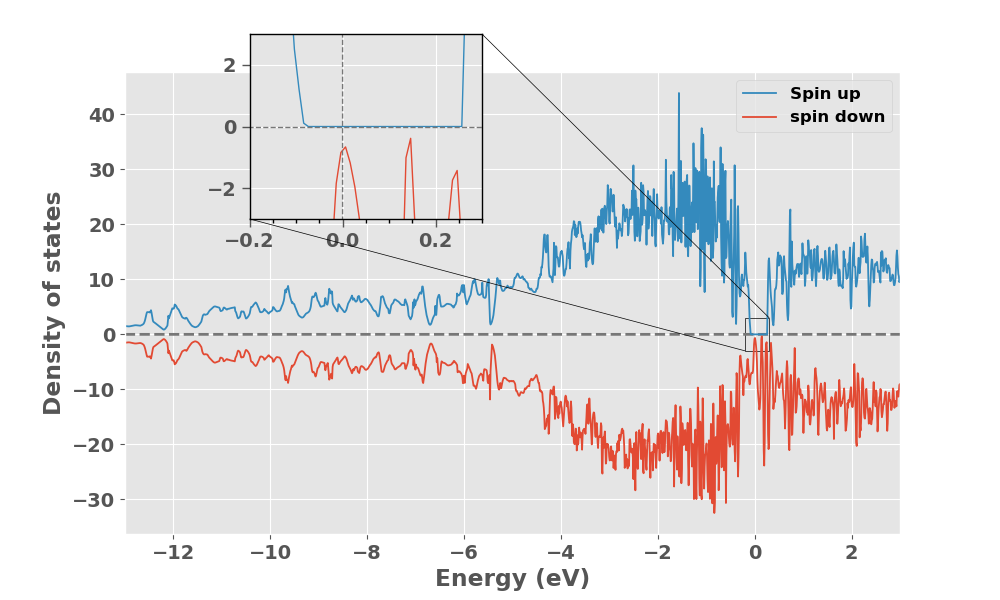
\includegraphics[width=.8\textwidth]{results/fesi2/D_TDOS.png}
	\caption{Density of states of SQS D \ch{(CrFeMnNi)Si2} with PBE.}
\end{figure}

Above we plot the electronic density of states of SQS D from calculations with the PBE GGA functional. This supercell and it's corresponding properties are emphasized for it's relative stability in the set. Being the most stable means it's the most representative structure of the potentially "real" material, and hence so are the properties of that SQS. From the DOS in figure 7.1 we discover that the structure is in fact a half-metal with a band gap around 0.4 eV in the spin up channel and a metal in spin down. In figure 7.2 bellow we plot likewise the density of states corresonding to the second utmost stable SQS B, here clearly displaying a band gap in both spin directions. 

\begin{figure}[H]
\centering
	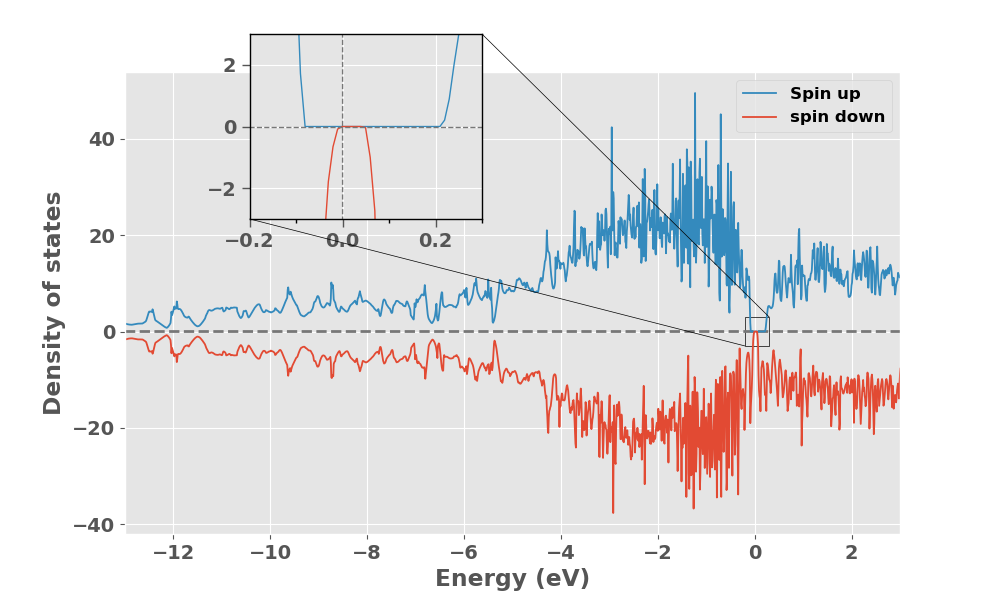
\includegraphics[width=.8\textwidth]{results/fesi2/B_TDOS.png}
	\caption{Density of states of SQS B \ch{(CrFeMnNi)Si2} with PBE.}
\end{figure}  

The density of states of the other SQSs can be seen in appendix .., the spin dependent band gaps can be seen in table 7.2, as determined from the calculated eigenvalues. In all 5 we find a trend of significantly greater band gaps in the spin up direction as seen in D, however the other also contain small nonzero gaps in spin down. This result can be related to the magnetic properties discussed above for the alloys. Contrary, the band gap in bulk \ch{FeSi2} is identical in both spins in accordance with the nonmagnetic character. 
 
\begin{table}[H]
\centering
\begin{tabular}{@{}cccc@{}}
\toprule
Structure  & Spin-up & Spin-down & Total  \\ \midrule
\textbf{A} & 0.0814  & 0.0522    & 0.0281 \\
\textbf{B} & 0.2932  & 0.0523    & 0.0523 \\
\textbf{C} & 0.2355  & 0.0343    & 0.0343 \\
\textbf{D} & 0.3386  & 0         & 0      \\
\textbf{E} & 0.3078  & 0.0495    & 0.0495 \\ \bottomrule
\end{tabular}
\caption{Band gap (eV) with PBE in spin up and spin down channels of CFMN (fesi2) SQSs}
\end{table}
  
Alike the bulk material, these gaps are indirect. It would have been instructive to visualize and analyze the energy bands by plotting the band structure. Unfortunately this is neither simple to perform or interpret in large supercells consisting of several elements and a large number of energy bands. One solution is to do band-unfolding, but given the complex structure and implementation of the special quasi-random structures method in VASP this proved too challenging for the scope of this project.To explain the result of SQS D in comparison to the other semiconducting SQSs of the alloy, we look at the calculated eigenvalues for the distinct supercell. Here it's seen that eigenstates transition between full to empty occupancy at energy band 124 in spin down and 129 in spin up, thus a difference of 5 bands between states in the different spins, this is also the case in the other SQSs. In particular of SQS D however is that for a majority of k-points the bands 124 and 125 contain occupancy values other than 1 and 0 for the spin down states. These are either non-physical values above 1 or negative, in other words indicating states are more than filled or less than empty. Or values in-between 1 and 0, meaning partially filled states (defect states). If we were to neglect these defect states and only consider bands where the occupancy is above 0.99 or bellow 0.01, the band gap of structure D remain consistent in spin up, but we now observe a band gap of around 0.05 eV in the spin down channel as well. This concept of defects in the forbidden energy gap is a well known factor of random alloys that is known to prohibit a band gap \cite{PhysRevLett.104.236403}. Again, this would have been extremely insightful to investigate with the help of a band structure diagram. The non-physical values is simply a consequence of using the tetrahedron method with Bloch corrections as numerical smearing, but poses no significant problems to the results. Interestingly we only find such values for spin channels also containing defect states. Furthermore the presence of such defect/non-physical states is found as the key divider between structures with and without a band gap also for the coming examples in this project.  
 
\section{Local and projected density of states}
  
\begin{figure}[H]
	\centering
	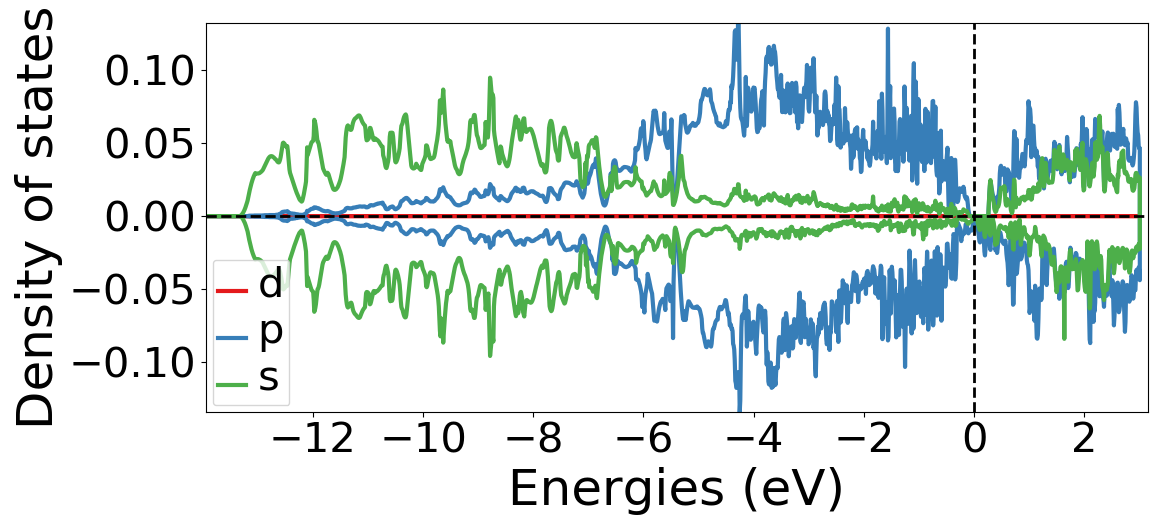
\includegraphics[width=.7\textwidth]{results/fesi2/D_LDOS_Si.png}
	\caption{Local density of states of Si (SQS D)}
\end{figure} 

\begin{figure}[H]
	\centering
	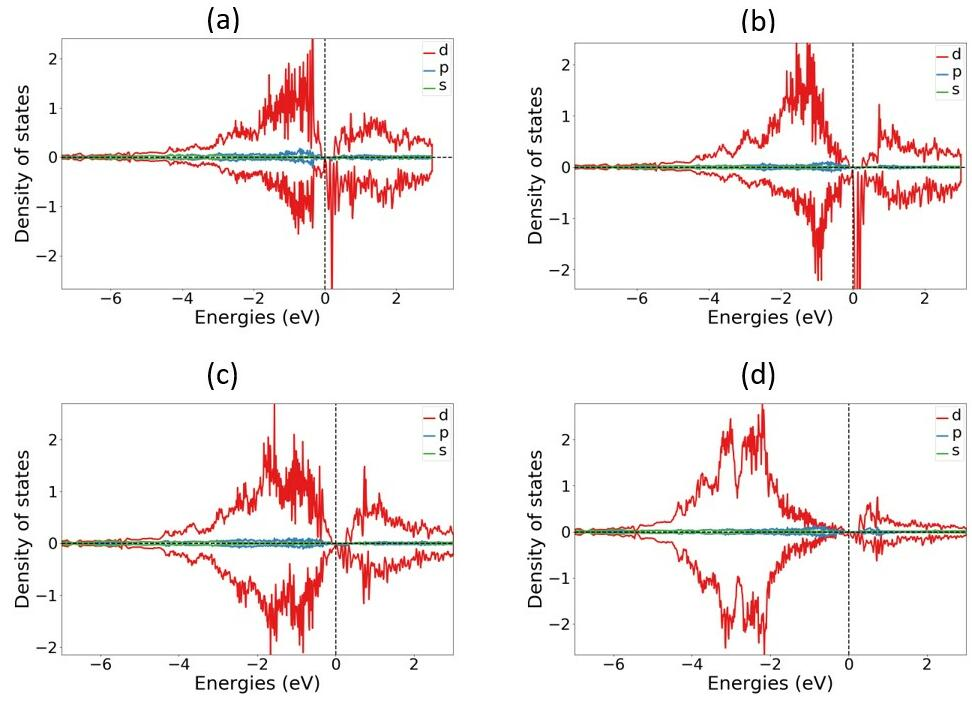
\includegraphics[width=\textwidth]{results/fesi2/D_LDOS.jpeg}
	\caption{Local density of states of (a) Cr, (b) Mn, (c) Fe, (d) Ni in SQS D.}
\end{figure}   
  
In the local density of states plotted in figure 7.3 we see that the s-electrons in Si occupy states in the lower energy regions and p electrons at slightly elevated energies closer to the Fermi energy, above $E_F$ states are occupied by both s and p electrons almost equally. Further, the local density of states of the transition metals chromium, manganese, iron and nickel in SQS D is displayed bellow in figure 7.4. In spin down, manganese is most dominant especially above $E_F$, but also bellow $E_F$. Likewise chromium show a strong presence above the Fermi energy in spin down. Both iron an Nicel show largest contribution at energies further from the Fermi energy, most notably bellow $E_F$. In the spin up channel we see a similar trend where chromium lie closest to $E_F$ followed by manganese then iron and lastly nickel at the lowest energies. Another interesting observation is that the the LDOS of iron and nickel is much more symmetric between spins, than Cr and Mn. Comparing to the LDOS of iron and silicon in bulk $\beta-$ \ch{FeSi2} \cite{doi:10.1063/1.346415} we find good agreement for both Fe and Si in this alloy .

\begin{figure}[H]
	\centering
	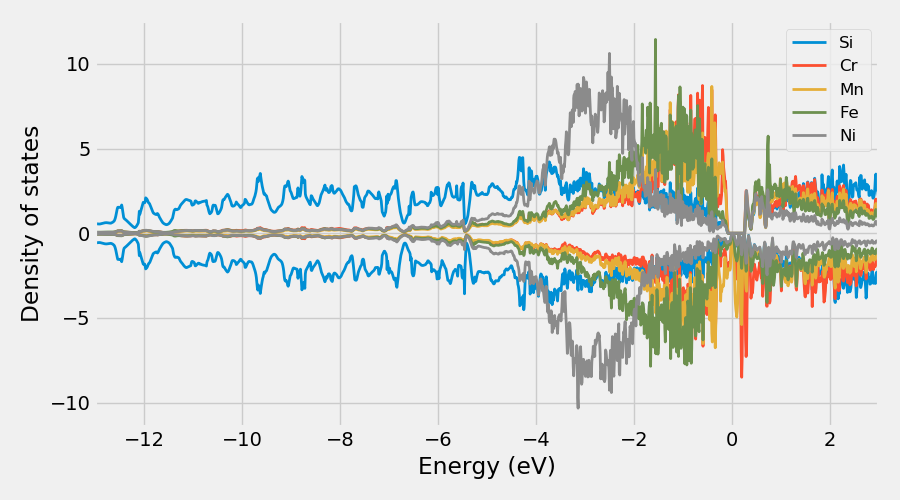
\includegraphics[width=.8\textwidth]{results/fesi2/D_PDOS.png}
	\caption{Projected density of states SQS D CFMN (fesi2) from PBE calculation}
\end{figure} 

Moreover the relative positions and interplay between 3d elements and silicon as shown in the projected density of states (figure 7.5) is in good agreement with observed trends in simpler Si-rich transition metal silicides \cite{lange1997electronic}. The electronic structure tends to be dominated by TM d electrons, and the valence band density of states are filled by non-bonding d states near $E_F$. The p-d hybridization between Si and TM elements typically fall about 6 eV bellow $E_F$ and Si $s$ states about 10 eV bellow. In our case we find that the Si states are pushed up closer to the fermi energy by random alloying of various 3d elements.    

  
\begin{figure}[H]
	\centering
	\begin{subfigure}{.45\textwidth}
			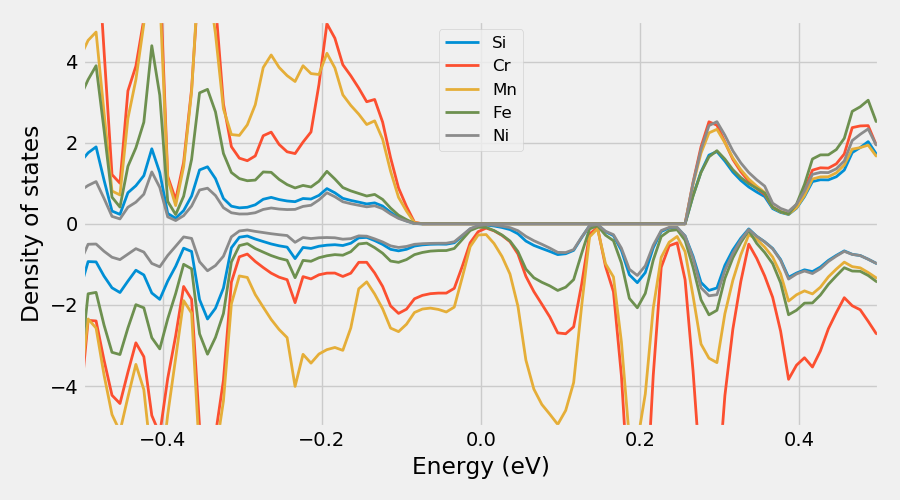
\includegraphics[width=\textwidth]{results/fesi2/D_PDOS_Ef.png}
			\caption{SQS D}		
	\end{subfigure}
	\hspace{0.5cm}
	\begin{subfigure}{.45\textwidth}
		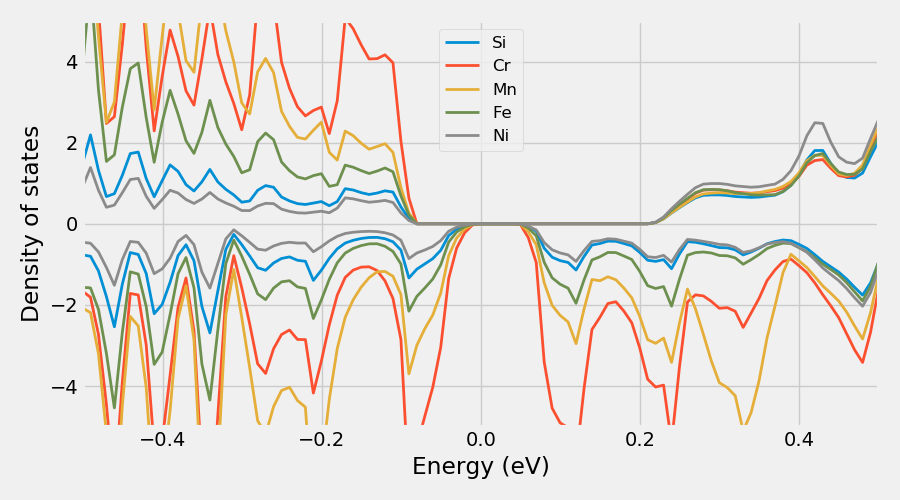
\includegraphics[width=\textwidth]{results/fesi2/B_PDOS_Ef.png}
		\caption{SQS B}		
	\end{subfigure}
	\caption{Projected density of states of SQS D and B around $E_F$}
\end{figure}

Above we have included the PDOS of SQS D and B but focused around $E_F$, from these figures we find that the spin down channel in D contain a more dominant presence of manganese especially, and some chromium as compared to the semiconducting SQS B.  

\section{Results from SCAN and HSE06 functionals}

As expressed previously in this work we invoke 3 level of depths GGA (PBE), meta-GGA (SCAN) and hybrid functional (HSE06) to determine the band gap of the SQSs. In table 7.3 we list the respective band gaps of these methods for all 5 SQSs of \ch{(CrFeMnNi)Si2}.

\begin{table}[H]
\centering
\begin{tabular}{@{}cccc@{}}
\toprule
Structure  & PBE    & SCAN   & HSE06  \\ \midrule
\textbf{A} & 0.0281 & 0.0000 & 0.0207 \\
\textbf{B} & 0.0523 & 0.0890 & 0.1808 \\
\textbf{C} & 0.0344 & 0.0690 & 0.0196 \\
\textbf{D} & 0.0000 & 0.0000 & 0.0000 \\
\textbf{E} & 0.0495 & 0.1048 & 0.0133 \\ \bottomrule
\end{tabular}
\caption{Band gap of CFMN (\ch{FeSi2}) SQSs with GGA (PBE), meta-GGA (SCAN) and hybrid-functionals (HSE06).}
\end{table}

The most obvious result of table 7.3 is that aside from SQS A, all 3 methods agree on the presence of the band gap. On the other hand, it's clear that the actual size of the gap is under some debate. We note the largest observed band gaps is largely associated with the SCAN functional in line with what is expected by involving more complex factors in the exchange-correlation functional, as discussed in section .. In contrast, by the same argument we would not expect that par SQS B, the overall smallest band gaps is found with the well-proven hybrid functional HSE06.
 
On the surface the results of table 7.3 point to sensible results from applying the SCAN functional, however we do make note of certain oddities under the surface. In SQS A the SCAN functional resulted in a zero total band gap, as opposed to 0.03 eV from PBE. In SQS B and E the band gap is increased with SCAN, but the properties of the gap is reversed compared to PBE. This can be seen for SQS E in figure 7.7 (a, b). In structures C and D this is taken a step further and reverse the spin polarization of the band gap, seen in figure 7.7 (c, d) for SQS C.
 
\begin{figure}[H]
	\begin{subfigure}{.5\textwidth}
		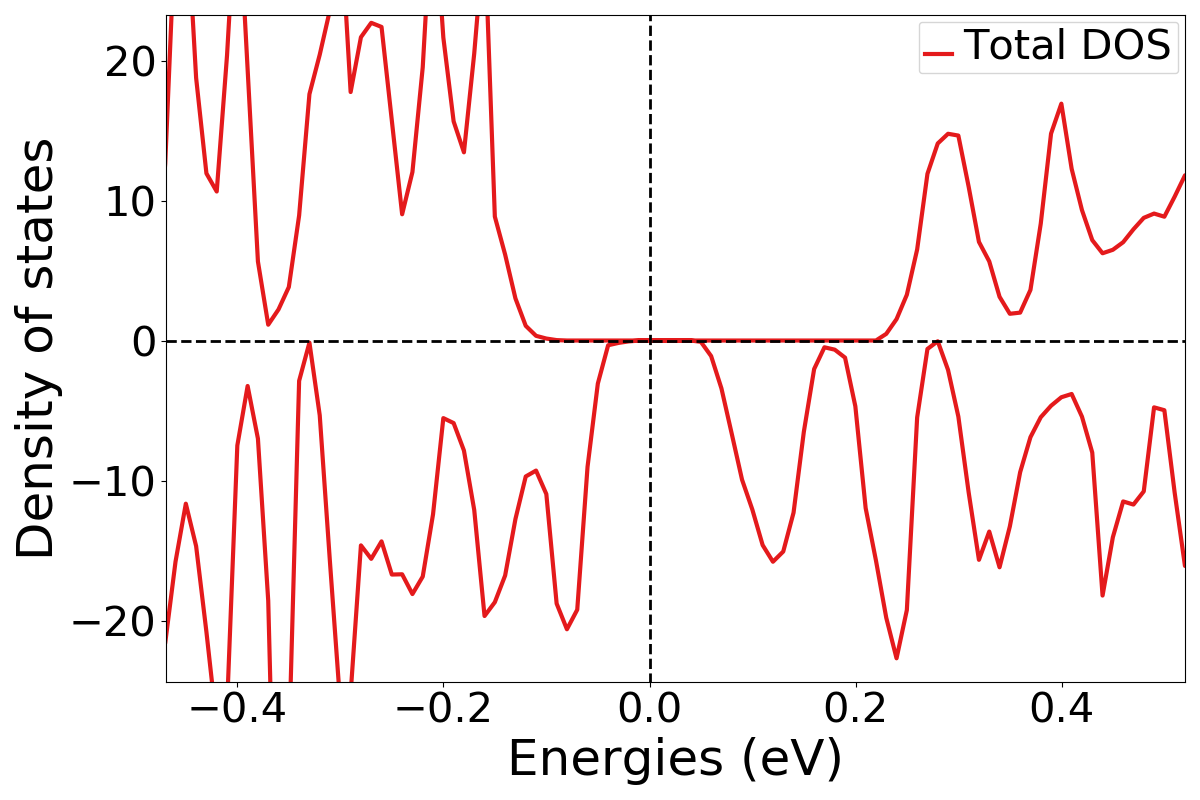
\includegraphics[width=\textwidth]{results/fesi2/E_DOS_pbe.png}
		\caption{SQS E PBE}
	\end{subfigure}
	\begin{subfigure}{.5\textwidth}
		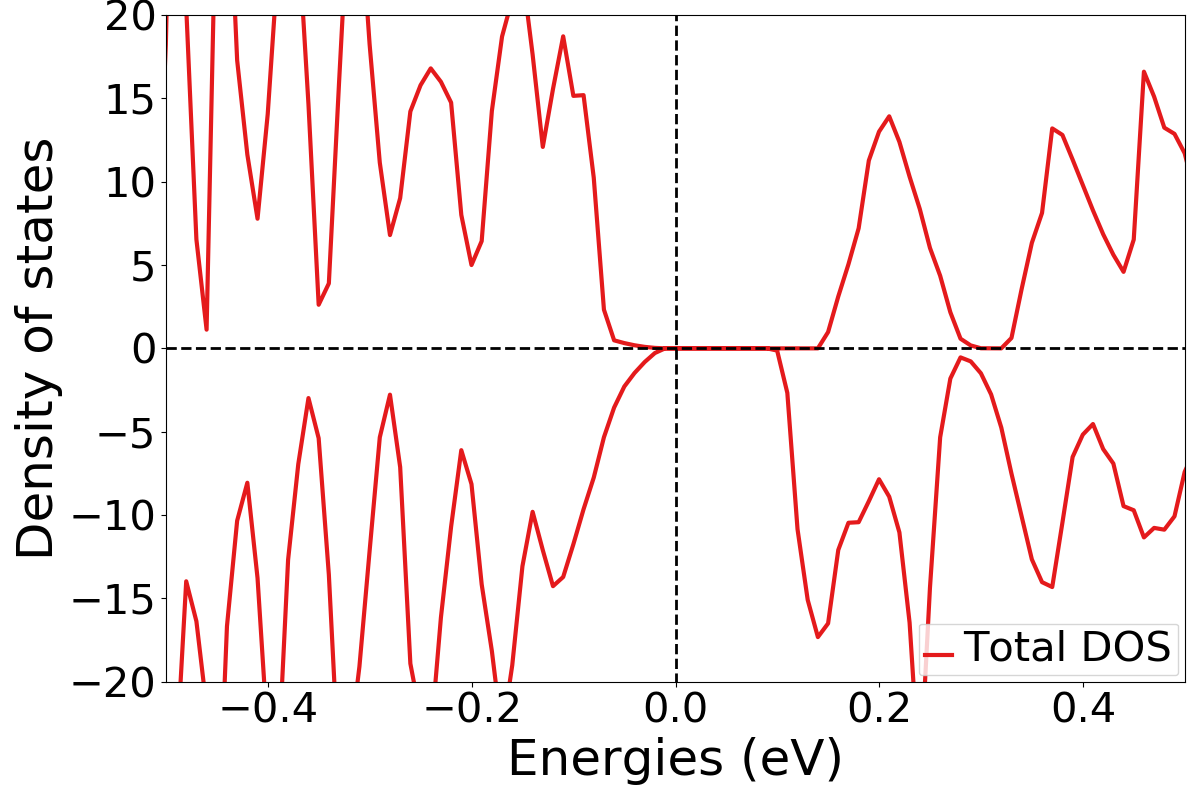
\includegraphics[width=\textwidth]{results/fesi2/E_DOS_scan.png}
		\caption{SQS E SCAN}
	\end{subfigure}
	\begin{subfigure}{.5\textwidth}
		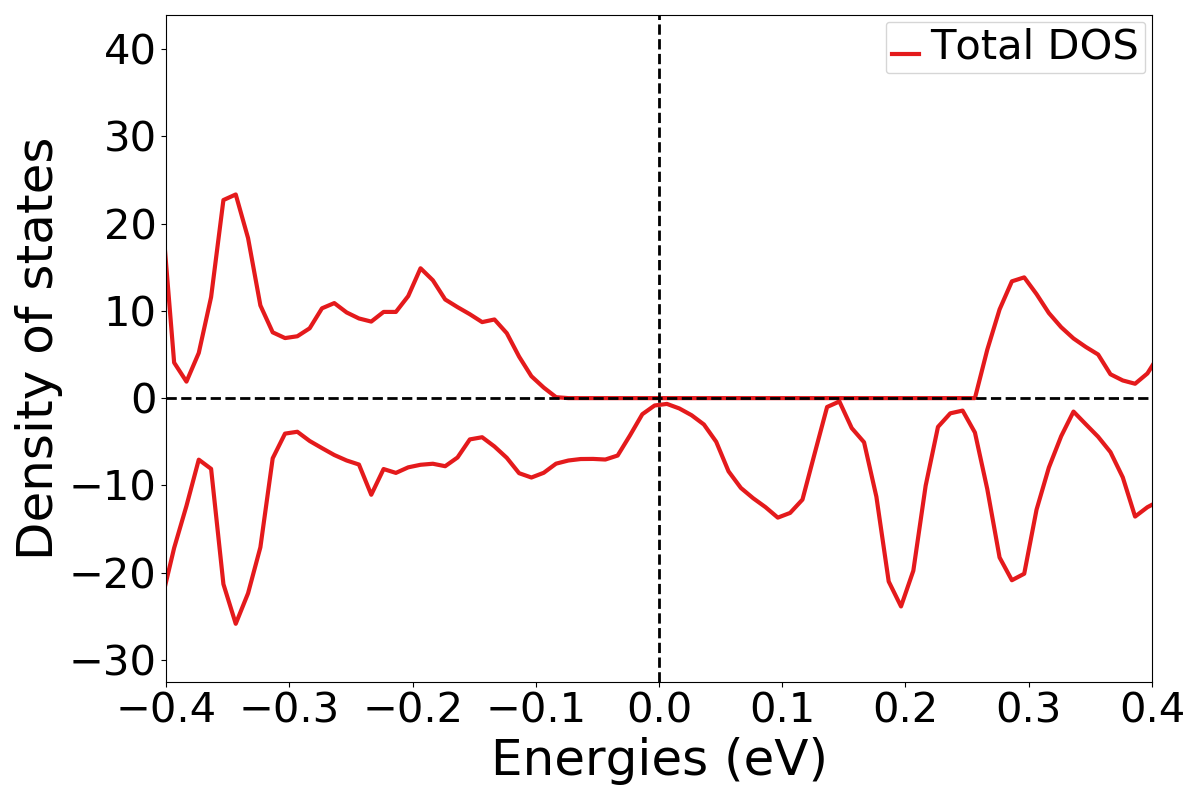
\includegraphics[width=\textwidth]{results/fesi2/D_DOS_pbe.png}
		\caption{SQS D PBE}
	\end{subfigure}
	\begin{subfigure}{.5\textwidth}
		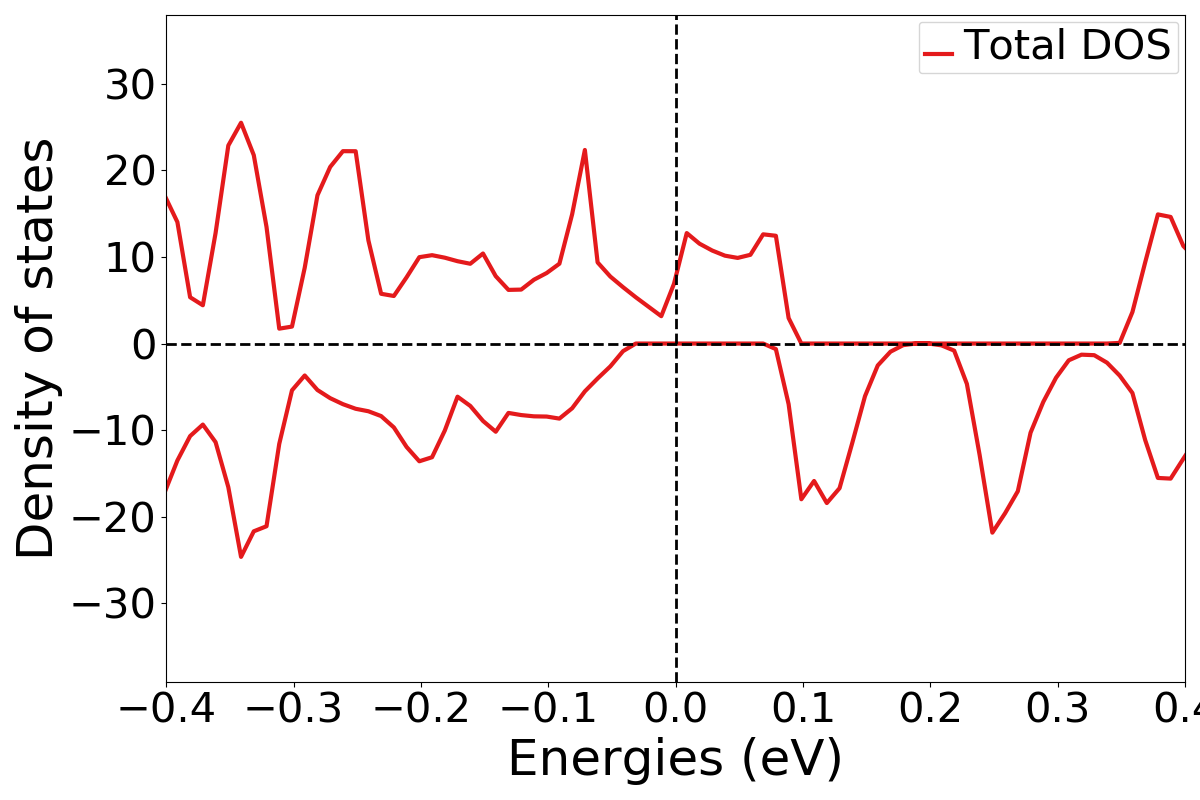
\includegraphics[width=\textwidth]{results/fesi2/D_DOS_scan.png}
		\caption{SQS D SCAN}
	\end{subfigure}
	\caption{Density of states illustrating the band gaps from PBE and SCAN calculations for SQS E and D.}
\end{figure}


In SQS B we find from calculations with HSE06 an increment tot the band gap to a value of 0.18 eV. This gap can be seen in terms of the density of states in figure 7.8. Compared to the other listed values of table 7.3 this is the sole case we obtain such a result from the HSE06 functional.   

\begin{figure}[H]
	\centering	
	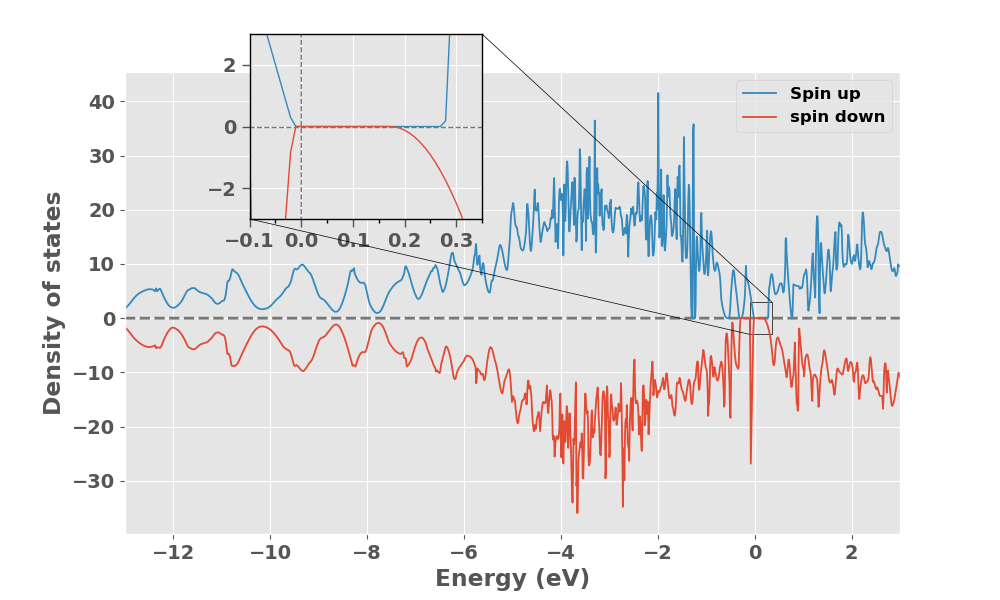
\includegraphics[width=.8\textwidth]{results/fesi2/B_TDOS_hse06.png}
	\caption{Density of states of SQS B with HSE06}
\end{figure}


Aside SQS B, we generally see good agreement between HSE06 and PBE calculations. In A we notice that the 0.02 eV band gap stems from a 0.7 eV gap in spin up and 0.02 eV in down. Likewise SQSs C, D, and E all exhibit large band gaps in spin up, 0.17, 0.37 and 0.55 eV respectively, and correspondingly very narrow spin down gaps of 0.032, 0, and 0.013 eV. The DOS of these SQSs can be found in appenidix \textbf{?}. Compared to the values in table 7.3 the HSE06 functional either compare or exceed the PBE band gaps in spin up and lessen in spin down, with the exception of SQS B (0.29 eV and 0.18 eV) where also the spin down gap is increased. As opposed to the SCAN functional that yielded dissimilar values to PBE in most cases.

\textbf{Change this to the correct figure}
\begin{figure}[H]
\centering
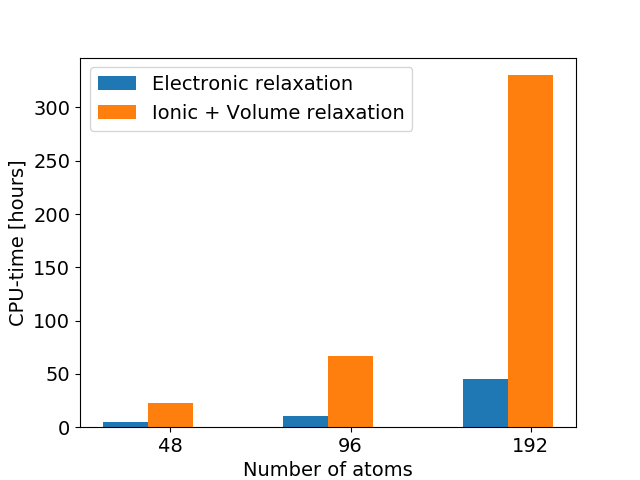
\includegraphics[width=.8\textwidth]{results/SQS_time.png}
\caption{Something}
\end{figure}


Discuss factors concerning the calculations.blablabla \\



Above we have plotted the computational cost in terms of CPU hours per CPU for the generalized gradient approximation, meta-GGA and hybrid functional. In relation to the topics covered in section 5.1 we see a clear trend in increased cost from more advanced functionals, with HSE06 taking about .. compared to PBE, while SCAN falls somewhere in-between. One of the reasons behind the large cost of HSE06 is as stated we had to perform such calculations in two subsequent iterations, firstly with Gaussian smearing and then secondly with TBC reapplying the calculated charge density. Keep in mind also that HSE06 utilized only halve the number of k-points compared to both PBE and SCAN. This could lead to artificially exaggerated band gaps from HSE06 as the low density of k-points could fail to encapsulate the exact minimum transition between the valence band and conduction band. But in most cases this does not seem to be a factor, with possibly the exception of the abnormally large band gap in SQS B. Regarding PBE and SCAN both of these have known limitations. As stated in section 5.1 PBE have difficulties for 3d elements particularly Ni, similarly SCAN is known to be limited in magnetic materials. The only functional with no known drawback is HSE06, the sole drawback of this functional is the computational demand as seen in figure 7.5.

\textbf{Rewrite}
As a conclusion the fact that all 3 functionals and five structures for the most part agree on the presence of a band gap is in itself an overwhelmingly positive result that allow us to state with high certainty that this hypothetical high-entropy silicide \ch{(CrFeMnNi)Si2} is in fact a semiconductor, or possibly a half-metal based on the results of the utmost stable SQS D. An additional point to this is that as covered in great detail in literature on first principles studies, the PBE functional underestimate the value of a band gap. For example in this project we determine the band gap of bulk $\beta-$ \ch{FeSi2}with PBE calculations to around 0.65 eV compared to the experimental value of 0.85 eV. For this reason any values of the band gap with PBE would with high probability be replicated/increased for the real material. Compared to the nonmagnetic bulk material we find these alloys to yield sensible results, here we create a random alloy that as known will introduce defect states and hence lower the band gap and further make the material magnetic. We observe that this is most apparent in spin down as the the spin up gap is more comparable to the values of the bulk material, but the down channel is metallic. In the next section we will look at the probability distribution functions before considering factors related to the special quasi-random methods in section 7.4. 


\newpage
\section{Probability distribution functions}
The probability distribution functions of SQS D and E can be seen bellow in figure 7.10, the PDFs corresponding to the remaining SQSs can be found in appendix .. . We include the PDFs of SQS D and B because as stated D is the most stable atomic configuration and hence the most representative of a potential real compound, and B to investigate distinctions between the half-metallic structure D and the semiconducting B which with HSE06 yielded substantial band gaps in both spins, recalling also that this is just very slightly bellow D in terms of stability. In the analysis we will put special emphasis on the nearest neighbor interactions since these are the most crucial in deciding the functional properties of a material. 
 
\begin{figure}[H]
	\centering
	\begin{subfigure}{\textwidth}
		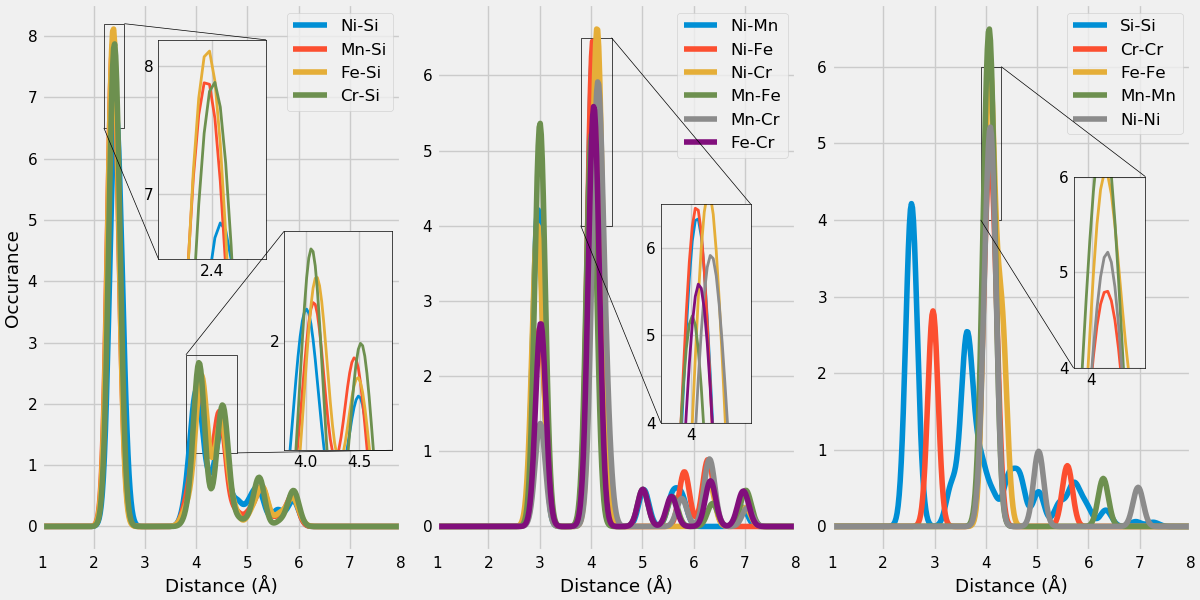
\includegraphics[width=\textwidth]{results/fesi2/D_PDF2.png}
	\end{subfigure}
	\begin{subfigure}{\textwidth}
		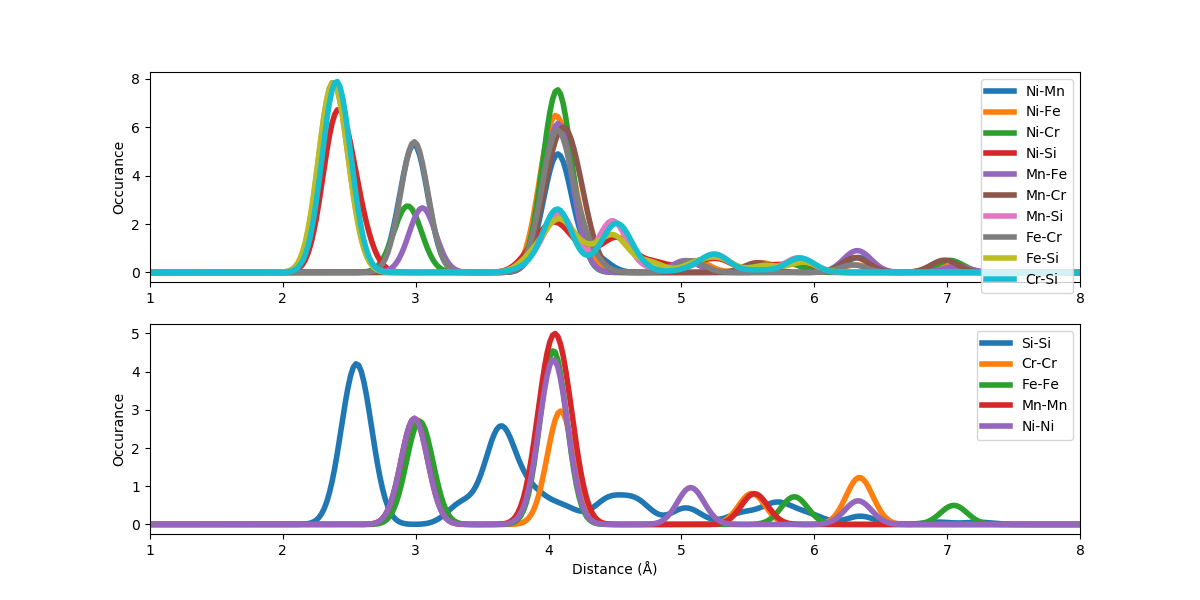
\includegraphics[width=\textwidth]{results/fesi2/B_PDF.png}
	\end{subfigure}
	\caption{Probability distribution function of SQS D (top) and B (bottom)}
\end{figure}

We see that the relative positions of the PDFs remain consistent though both SQSs. With the aid of the ICSD (insert citation), we can compare the figure .. to the expected PDFs based on a number of experiments from a host of different compounds. As our compound contain a total of 15 different bonds, comparing each one to the ICSD values would be an exhaustive process. For our purpose we are satisfied by comparing the 4 different metal-Si bonds. We find that the preferred bond-length of TM-Si is observed at two values, the most dominant being the shorter of the two. For Fe-Si these are between 2.25-2.75 and 4-5, Mn-Si 2.25-2.75 and 3.5-5. Ni-Si lie between 2.25-2.5 and 3.85-5 and Cr-Si between 2.35-2.65 and 4-5.Clearly, the PDFs of the alloys are in good agreement with the listed values for Tm-Si bonds, with the most occurring bond length falling at around 2.4 Å for all TMs, and lesser occurrence between 4.0 - 4.5 Å. The height of the respective peaks is somewhat consistent in both structures, other than slightly reduced Fe-Si occurrence at 2.4 Å in B.

In contrast to the TM-Si bonds, we observe several distinctions between metal bonds in SQS D and B. Covering all would be tedious and not to insightful, instead we emphasize the bonds of Mn and Cr as this is where we found the biggest discrepancy in the PDOS. From the different TM-TM bonds (middle) of figure 8.8 we observe that the Mn-Fe bonds are most occurring at short distances in D and bigger distances in B, meaning that manganese and iron atoms are placed further from each other in structure D. \textbf{correct?} Similarly the bonds between Cr and Fe   indicate that these atoms lie closer in B than D. In contrast the nickel and manganese/chromium bonds point to a closer distance in B for Ni-Mn and Ni-Cr in D, and a greater distance between Ni and Mn in D and Ni and Cr in B. \textbf{Litt kronglete kanskje?} In terms of the homogeneous bonds, the properties of both Cr-Cr bonds and Mn-Mn bonds are more or less alike in both structures besides some majority at shorter distance in D (The red Cr-Cr line at 3Å is underneath the grey Ni-Ni line in B in figure 8.8 (bottom right)). A more significant distinction is that both Ni-Ni and Fe-Fe bonds are found at 3 Å and 4 Å in B, but exclusively 4 Å in D.    

Both the Fe-Fe and Ni-Ni bonds are in better agreement with the ICSD histograms, as the most occurring distance for these bonds are between 4-4.9 Å and additionally around 2.5 Å. \textbf{More comparisons to ICSD, ask O.M}. As a conclusion on the PDFs of this compound, we locate a pattern where the Si-Si bonds are identical and only very minor differences between TM-Si bonds in SQS D and B. This is a result of how the structures are generated with the SQS method. In th FeSi2 structure the silicon atoms are placed as before in the new supercells, but the TM elements are "randomly" distributed. Thus, it's reasonable that also here we would find the major differences between SQSs in the PDFs. 

\newpage
\section{SQS size}

Lastly a precise determination of the exact value of the band gap would requiere much more effort. Recalling the concerns of the special quasi-random structures, we know that one problem is the large possible number of configurations. Here we select only a span of 5 and we find that the band gap varies greatly between all 5 but show the same characther. Thus we should have performed a larger search over more configurations. Additionly also the SQS size is relevant, here we have only tested a 48 atom model, but as section .. stated often much larger SQSs are required to reach convergence and accuratly model the disordered structure of HEA. At the same time this is not a true disordered structure, the Si atom contain some order and this is not really a typicial HEA so maybe this is not as important.

In this project we have made calculations of a type of supercell and SQS model. This model consisted of 48 atoms and have a volume of $700 Å^3$ before structural relaxation. This was done for two reasons, firstly it allowed for the use of more complex XC-functionals, and secondly enabled a broad study of distinct permutations and compositions. However, as covered in section 4.2 or something the results of the SQS model is known to show a sensitivity to the size of the model. For this reason we include the results of 96 and 192 atom SQSs of \ch{CrFeMnNiSi2} with volume $1200 Å^3$ and $2400 Å^3$ respectively. Bellow in figure .. we show the increased computational burden in terms of cpu-hours from performing both structural and ionic relaxation as well as a single electronic self-consistent calculation with PBE GGA of the distinct SQSs. 

\begin{figure}[H]
\centering
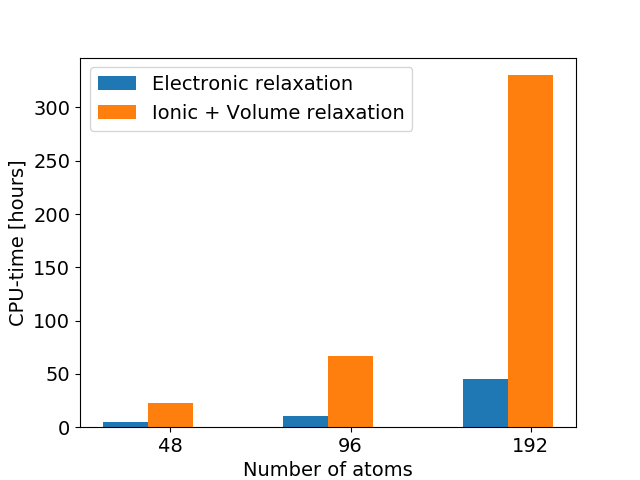
\includegraphics[width=.8\textwidth]{results/SQS_time.png}
\end{figure}

\begin{table}[h!]
%\centering
\hskip-2cm\begin{tabular}{@{}cccccc@{}}
\toprule
       & \multicolumn{2}{c}{Total energy/atom (eV)} & Enthalpy of formation (eV) & \multicolumn{2}{c}{Final magnetic moment ($\mu_B$)} \\ \midrule
48 atoms & - 6.6105 & .. & -11.5000 & 0.0833 & 0.0000    \\
96 atoms & - 6.6092  & 0.0021 & - 22.8752  & 0.0708  & 0.0114     \\
192 atoms & - 6.6123  & 0.0022 & - 46.6654 & 0.0761 & 0.0171     \\ \bottomrule
\end{tabular}
\caption{Mean and stadard deviation of the total energy and magnetic moment per atom, plus enthalpy of formation of the listed mean energies (\ch{FeSi2}).}
\end{table}


\begin{figure}[H]
\begin{subfigure}{\textwidth}
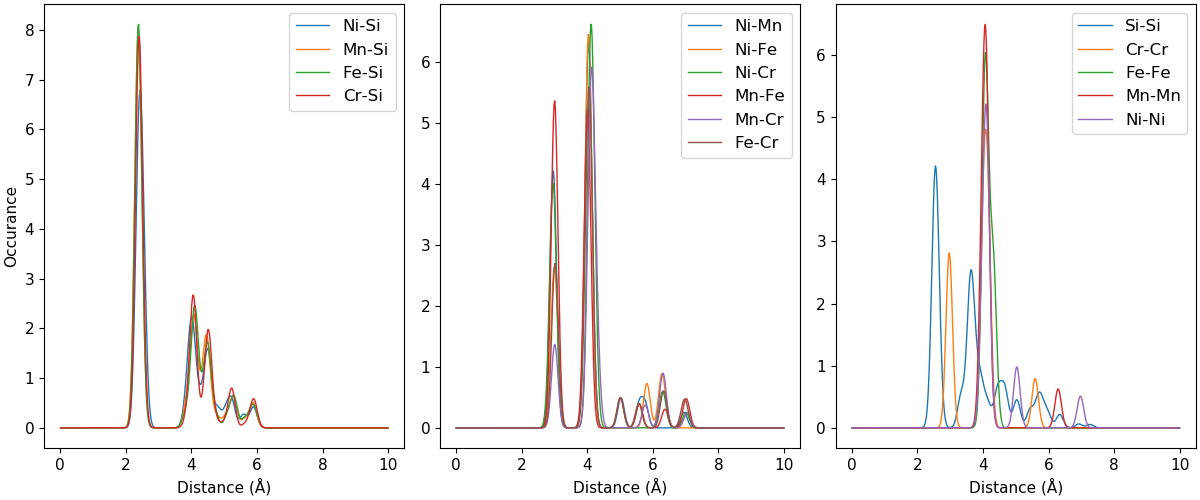
\includegraphics[width=\textwidth]{results/PDF48.png}
\end{subfigure}
\begin{subfigure}{\textwidth}
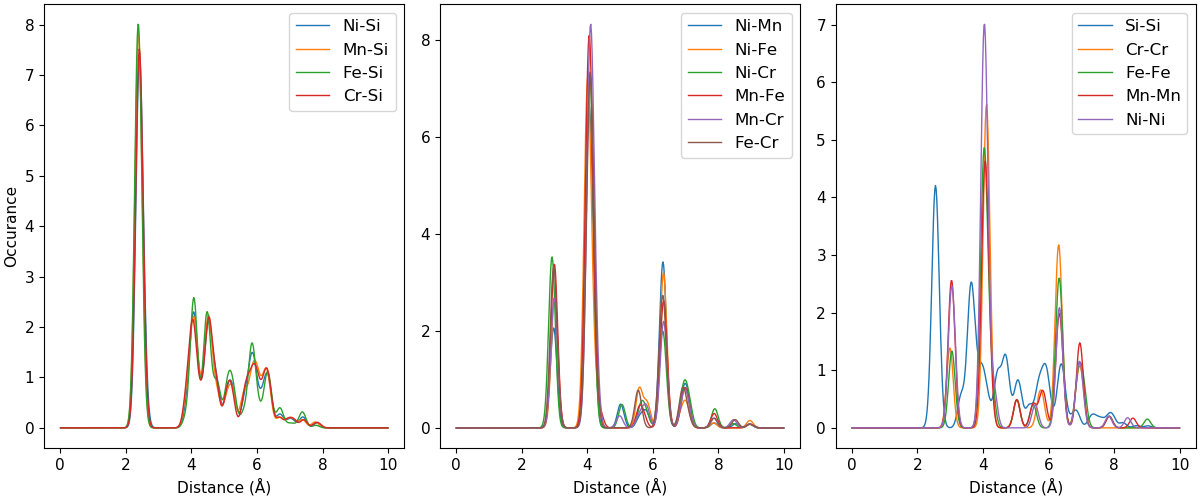
\includegraphics[width=\textwidth]{results/PDF96.png}
\end{subfigure}
\begin{subfigure}{\textwidth}
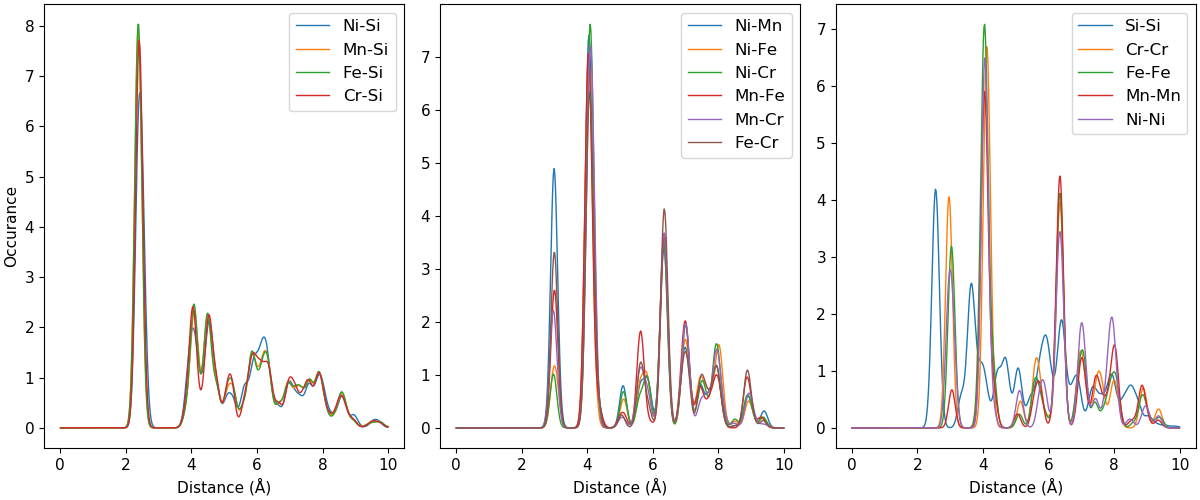
\includegraphics[width=\textwidth]{results/PDF192.png}
\end{subfigure}
\end{figure}


\begin{table}[H]
\centering
\begin{tabular}{@{}ccccc@{}}
\toprule
                                                     &   & Spin up (eV) & Spin down (eV) & Total (eV) \\ \midrule
\multicolumn{1}{c|}{\multirow{5}{*}{\textbf{48 atoms}}}   
												  & A & 0.0815                & 0.0521                  & 0.0281              \\
\multicolumn{1}{c|}{}                                & B & 0.2932                & 0.0523                  & 0.0523              \\
\multicolumn{1}{c|}{}                                & C & 0.2355                & 0.0343                  & 0.0343              \\
\multicolumn{1}{c|}{}                                & \textbf{D} & 0.3386                & 0                       & 0                   \\
\multicolumn{1}{c|}{}                                & E & 0.3078                & 0.0495                  & 0.0495              \\ \midrule
\multicolumn{1}{c|}{\multirow{5}{*}{\textbf{96 atoms}}}   
                                                     & \textbf{A} & 0.1705                & 0.0442                  & 0.0367              \\ 
\multicolumn{1}{c|}{}                                & B & 0.1386                & 0.0270                  & 0.0270                   \\
\multicolumn{1}{c|}{}                                & C & 0.1347                & 0.0363                  & 0.0075                   \\
\multicolumn{1}{c|}{}                                & D & 0.0892                & 0.0398                  & 0.0398                   \\
\multicolumn{1}{c|}{}                                & E & 0.1610                & 0                       & 0                        \\ \midrule
\multicolumn{1}{c|}{\multirow{5}{*}{\textbf{192 atoms}}}
	 									           & A & 0.1197                & 0.0321                  & 0.0321                   \\
\multicolumn{1}{c|}{}                                & B & 0.1444                & 0                       & 0                        \\
\multicolumn{1}{c|}{}                                & C & 0.1867                & 0                       & 0                   \\
\multicolumn{1}{c|}{}                                & D & 0                     & 0                       & 0          \\
\multicolumn{1}{c|}{}                                & \textbf{E} & 0.0131                & 0.0184                       & 0.0131                   \\ \bottomrule
\end{tabular}
\caption{Total and spin dependent band gap of 4 permutations of CFMN (fesi2) with PBE GGA calculation. The structures that are excluded from this list either failed in calculations, or does not show any band gap.<}
\end{table}
